\section{Sound and its representation}

\begin{frame}{What is sound?}
  \begin{itemize}
  \item Sound is caused by vibrations
  \item Vibrations create waves, travelling through a medium
  \item Humans perceive acoustic waves with their ears, as eardrum are
    vibrating, converting the signal for the brain
  \item It is usually represented as a sine wave, however, it is a
    longitudinal wave (compression/rarefaction) in air and water and a
    transversal wave in solids.
  \end{itemize}
  \begin{center}
  \includegraphics[width=0.6\textwidth]{slides/audio-sound/CPT-sound-physical-manifestation.pdf}
  \end{center}
\end{frame}

\begin{frame}{Sound characteristics}
  \begin{itemize}
  \item Sound waves have a frequency, measured in Hertz (Hz), this is
    the pitch of the sound.
  \item They also have an amplitude, measured in decibels (dB), this
    is the loudness of the sound.
  \item Multiple waves of different frequencies and amplitude combine
    to create the actual sound with different qualities and timbre.
  \end{itemize}
  \begin{center}
  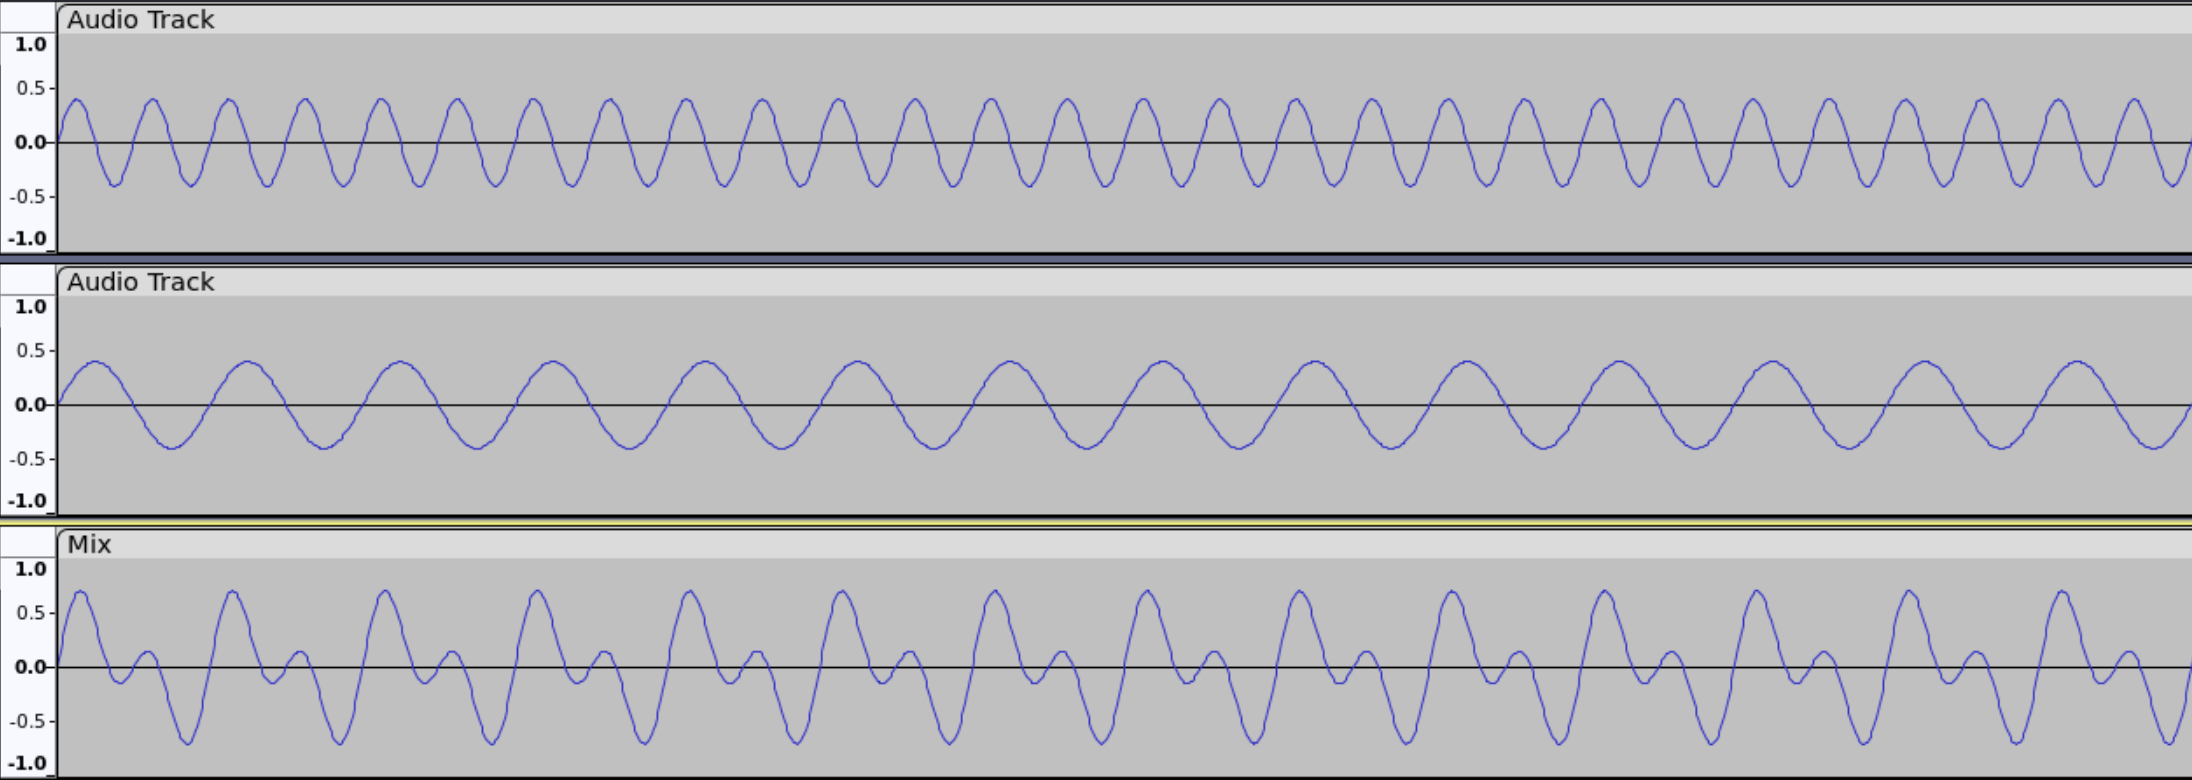
\includegraphics[width=0.8\textwidth]{slides/audio-sound/sound-compose.png}
  \end{center}
\end{frame}

\begin{frame}{Sound digitization - samples}
  \begin{itemize}
  \item Sound waves are continuous curves composed of a infinite
    number of points.
  \item For any point on the curve, it is possible to measure the
    audio level of this point.
  \item This is a sample. We can then take samples at regular interval
    to have a digital representation of the curve.
  \end{itemize}
  \begin{center}
  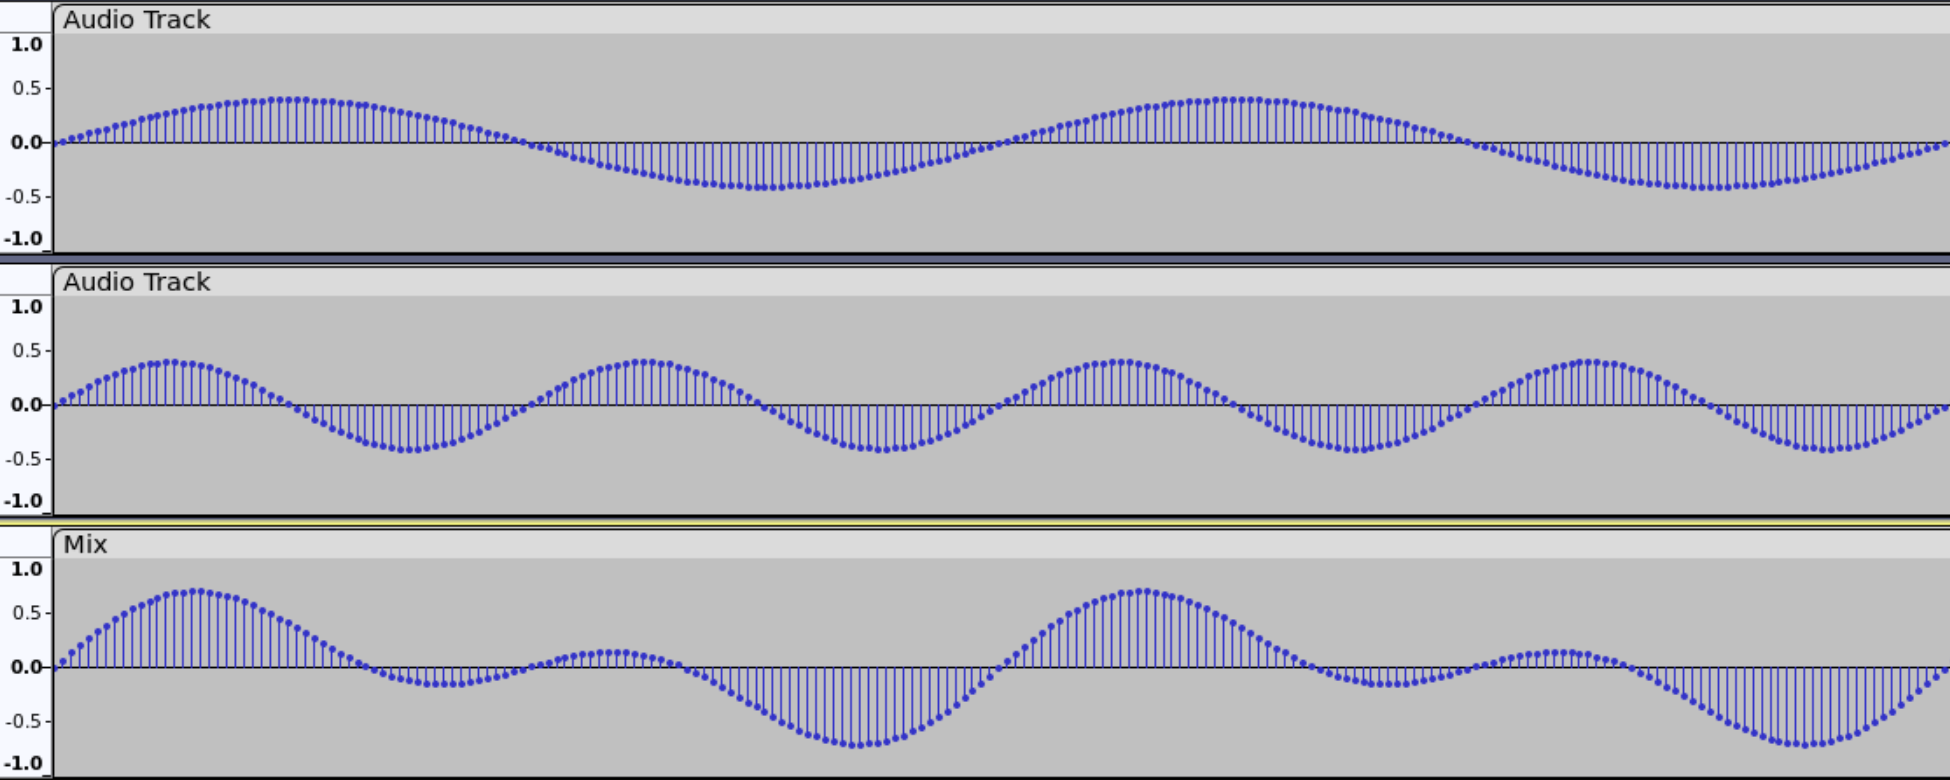
\includegraphics[width=0.8\textwidth]{slides/audio-sound/sound-samples.png}
  \end{center}
\end{frame}

\begin{frame}{Sound digitization - sample rate}
  \begin{itemize}
  \item The sample rate, or sampling frequency is the number of
    samples taken per seconds.
  \item If the sampling frequency is too slow, we may have aliasing
    issues were the sampled signal doesn't match the analog signal.
  \item The \textbf{Shannon-Nyquist theorem} states that the sampling
    frequency needs to be at least twice the maximum signal frequency
    to accurately digitize a signal.
  \item The Human ear can hear sound frequencies between approximately
    20~Hz and 20~kHz.
  \end{itemize}
  \begin{center}
  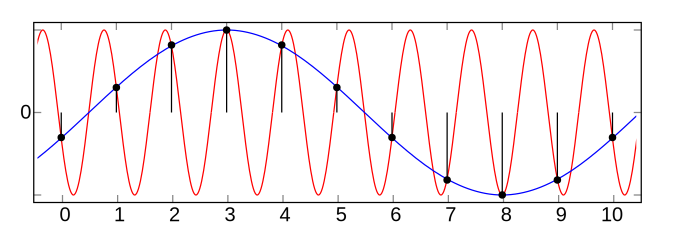
\includegraphics[width=0.6\textwidth]{slides/audio-sound/aliasing-1d.pdf}\\
  \textit{\small Aliasing example, the sampled signal is in blue}
  \end{center}
\end{frame}

\begin{frame}{Sound digitization - sample size}
  \begin{itemize}
  \item The sample value varies from 0 to the maximum amplitude value.
  \item If the amplitude is 1.0, then it varies from -1.0 and 1.0
  \item The sample size, in bits, then defines the resolution.
  \item Common sample sizes are 16 and 24 bits.
  \item 8 bits is getting very rare due to the poor audio quality and
    32 bits samples can be used when specific alignment is required.
  \end{itemize}
\end{frame}

\begin{frame}{Sound digitization - sample format}
  There are multiple ways to store samples in memory or on disk:
  \begin{itemize}
  \item as signed integers
  \item as unsigned integers
  \item as floating points
  \end{itemize}
  Also, they can be stored in little-endian or big-endian order.
  For 24bit samples, packing can also differ: either they are packed
  on 3 bytes or they can be packed in a 32bit integer with the most
  significant byte being ignored.
\end{frame}

\begin{frame}{Sound digitization - conclusions}
  \begin{itemize}
  \item We can then store sound as a sequence of samples and the
    specific sample rate that was used.
  \item This method is called Linear Pulse-code modulation or LPCM.
  \item A sampling rate of about 40kHz is needed.
  \end{itemize}
\end{frame}

\begin{frame}{Sound digitization - example WAV}
  WAV is a format based on RIFF and has the following header:
  \begin{center}
  \fontsize{8}{9}\selectfont
  \begin{tabularx}{13cm}{c|c|X}
    Position & Value & Description \\
    \hline
    1 - 4 & “RIFF” & RIFF FOURCC code \\
    5 - 8 &  & File size in bytes, minus 8 (32-bit integer). \\
    9 -12 & “WAVE” & WAVE FOURCC code \\
    13-16 & “fmt " & Format chunk marker. Includes trailing null \\
    17-20 & 16 & Length of format data, 16 for PCM \\
    21-22 & 1 & Audio format, 1 for PCM \\
    23-24 & 2 & Number of channels \\
    25-28 & 48000 & Sample rate \\
    29-32 & 176400 & Byte rate = (Sample rate * BitsPerSample * channels) / 8. \\
    33-34 & 4 & BlockAlign = (BitsPerSample * Channels) / 8 \\
    35-36 & 16 & Bits per sample \\
    37-40 & “data” & Data chunk header \\
    41-44 &  & Size of the data section in bytes \\
  \end{tabularx}
  \end{center}
\end{frame}

\begin{frame}{Sound digitization - example WAV}
  \begin{center}
  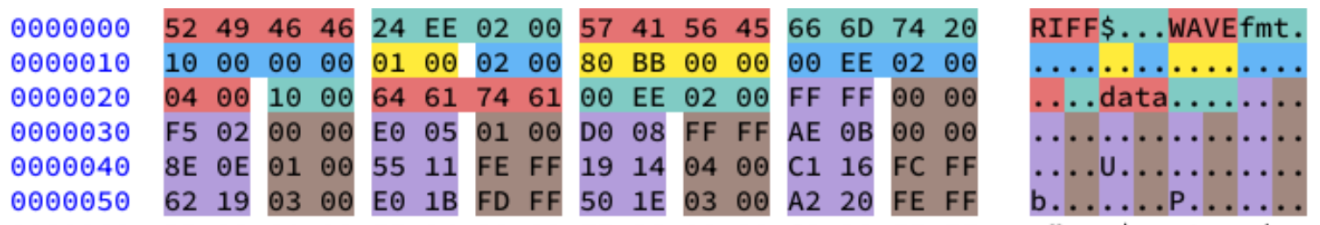
\includegraphics[width=\textwidth]{slides/audio-sound/RIFF_WAVE.png}
  \end{center}
\end{frame}


